\documentclass[a4paper]{article}
\usepackage[hmargin=1in, vmargin=1in]{geometry}
\usepackage{makeidx}
\usepackage{fancyhdr}
\pagestyle{fancy}
\usepackage[pdftex]{graphicx}
\usepackage{amsmath}
\usepackage{listings}
\makeindex
\begin{document}
\begin{center}
\title{Three dimensional coordinates into two dimensional coordinates transformation}\\
\author{Edward Gerhold}
\city{Berlin, Germany}
\date{\today}
\maketitle

Version 0.2.7 (the is getting reworked paper)\\
\textbf{Remark} This text may or may not contain logical errors, typos,
unclear phrases, remarks, during development. But this document is living
and being edited.

}\\

\end{center}


\tableofcontents\\

\section{Introduction}

On a piece of paper you see three coordinate axes pointing into three
directions in space. In reality these vectors are two dimensional. Because
they point into three directions on the paper, and not into the real space.\\

\begin{figure}[ht]
\label{ijksystem}
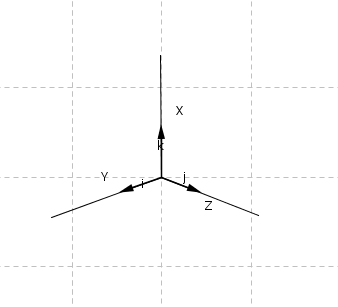
\includegraphics[scale=2]{ijksystem.png}\\
\caption{Picture of a 3-D coordinate system with ijk-vectors on the axes pointing
into three directions. See \cite{Corral1} for introduction.}
\end{figure}

In this document we will design a (pseudo-) basis for the coordinate transformation. 
A basis is multiplied with the values of the coordinates to move for each component 
a piece, to end the move on the correct new point.
In the case of cosines and sines, we move left and right and up and down, to 
tell you directly, what happens, when we multiply the coordinates with the matrix.\\

\textbf{What we will do in the document}

\begin{enumerate}
\item Choose angles for our coordinate axes around the unit circle to lay out three axes.
\item Write down the basis vectors for each coordinate axis
\item Assemble a matrix with the vector basis for a point by point transformation.
\item Read the example source code for a computer function, which is exactly two lines long. One for the new $x$ and one for the new $y$.
\item Derive the generic case of transforming coordinate systems down to the plane.
\end{enumerate}

\section{Designing a 2x3 transformation basis}

\subsection{The $_n$ index for $_x,_y,_z$ with $_x=1$, $_y=2$ and $_z=3$}

The index $_n$ in $r_n$, $\varphi_n$, $\vec{e}_n$ is the index for $_x$,$_y$,$_z$. For example $\varphi_n$  stands $\varphi_x, \varphi_y, \varphi_z$. $r_n$ stands for $r_x$, $r_y$ and $r_z$. $\vec{e}_n$ is for $\vec{e}_x$, $\vec{e}_y$, $\vec{e}_z$ It is possible, that in the formulas $x,y,z$ and $1,2,3$ may be used interchangeably. For example, when summing up the products of the coordinate componentents with basis components, this happens. The formula is $\sum_{i=1}^{2}\vec{x}_i\vec{e}_i$, which is a sum of $x,y,z$ and the $\cos \varphi_n$ terms in the first components of $\vec{e}_n$ for $x'$ and a sum of $x,y,z$ and the $\sin \varphi_n$ terms in the seconds components of $\vec{e}_n$ for $y'$.

\subsection{$\varphi_n$ the angles for the coordinate axes}

Why do we need angles? May be the first question. My answer is, we will arrange the basis vectors, 
easily around a circle by their angle. Since they are two dimensional. Instead of guessing wild numbers.\\

First draw three axes of a 3-D coordinate system on a piece of paper. Draw the horizontal x-Axis through the origin of the drawn coordinate system. You could directly add the y-axis, to see a 2-D coordinate system carrying your two dimensional 3-D system. A system with three vectors pointing into three directions, originating in the origin of the real R^2 space.\\

Each of the three vectors has an angle, counted from the horizontal positive x-axis, going counterclockwise around the origin. The
angle between the axes themselves isn´t what we want. We want the angle beginning on the real 2-D x-axis, to feed the cos and sin functions with, when calculating the real numbers of each basis vector.\\

In this document, i will call the angles $\angle \varphi_n$ or just $\varphi_n$. If they are measured in degrees or radians depends
on the cosine and sine functions you use. And on how you would like to read your own definition.

Let $\varphi_n$ be the set of axis angles, one for each axis. I put them into a set in this document to simplify the access by
using the index $_n$ together with $_x, _y, _z$ or $1,2,3$. $\varphi_x$ or $\varphi_1$ is the angle of the x-axis. $\varphi_y$ or $\varphi_2$ is the angle of the x-axis and $\varphi_z$ or $\varphi_3$ is the angle of the x-axis. 


\begin{displaymath}
\varphi_n := \{\varphi_x, \varphi_y, \varphi_z\} = \{ \varphi_1, \varphi_2, \varphi_3 \}
\end{displaymath}

We will need the three angles for the axes shortly. So don´t forget it over the next lines.


\subsubsection{Degrees or radians?}

Depending on the cosine and sine functions and the input value for the angles, you may have to convert the degrees to radians, or
the other way round, the radians to degrees. For example, the JavaScript Math.cos and Math.sin functions take the values in radians.\\

\begin{example}
\textbf{Example}
The function rad converts degrees to radians, it´s useful for computer functions taking radians.
\begin{displaymath}
\text{rad}(\phi) := \frac{\pi}{180} \times \phi, \phi \in \mathbb{R}
\end{displaymath}


Here is an example of three angles. The three axes have an angle of 120 degrees between each. But since we start counting counterclockwise and from the real horizontal axis of the plane, the angles are 210, 330, 90 in degrees, respectivly. And
because of the cosine and sine functions taking radians, we convert the values to radians.
 
\begin{displaymath}
\varphi_x = \text{rad(210)}, \varphi_y = \text{rad(330)}, \varphi_z = \text{rad(90)}
\end{displaymath}

\begin{displaymath}
\varphi_x &= \frac{\pi}{180} \times 210 &= \frac{7\pi}{6},  
\varphi_y &= \frac{\pi}{180} \times 330 &= \frac{11\pi}{6}, 
\varphi_z &= \frac{\pi}{180} \times 90 &= \frac{\pi}{2} 
\end{displaymath}
\end{example}


\textbf{Example}
The function deg converts the other way round and from radians to degrees. You multiply your value with the reciprocal of PI/180, namely 180/PI and get the other way round.
\begin{displaymath}
\text{deg}(\phi) := \frac{180}{\pi} \times \phi, \phi \in \mathbb{R}
\end{displaymath}

If you would like to get hands on angles, cosines, sines, or need a refresher, \cite{Corral2} is a good choice.

\subsection{$r_n$ is the length of the unit on each axis}

Before i show you the three vectors, and how to use them, we have to clear another piece of information belonging to each
basis vector. In this document it is called $r_n$. The r is from radius. And it stands for the length of the basis vector.
The length of the basis vector defines, how far a point in this direction will go by one unit.\\

The $r$ originates from radius from the unit circle and from the parametrization of (x,y) via cosine and sine. 
In polar coordinates the cosine and sine are multiplied with r. Also to change the length of the hypotenuse, 
the vector $\vec{r}$, which is the third side to a triangle by cosine, sine and r. 
If r is left away, the length of the basis vector is 1. Or in other words, the distance $d((0,0),(x,y))$ from the origin to $(x,y)=($$r \cos \varphi$$, $$r \sin \varphi$$)$ is $1$, if $r=1$ or if r is left away completely.\\

Pay attention to this point now, to keep the affine transformation, especially under rotation, correct. You should give all three
axes the same r-value. I will define them in this document as $r_n$ with one $r_x, r_y$ and $r_z$ for each coordinate axis,
to keep it complete. But if you would like to change the units on your objects, i have to recommend, that you apply a local
3x3 basis with the disjoint unit lengths. This will keep the rotation correct. In the other case, the object would suddenly
stretch the head, if you rotate it to the side, where the unit for example is longer.\\

So for the coordinate system, the best setting is $r_x = r_y = r_z$. Keeping them equal, you can rotate it realistic. But you
don´t need to keep the unit length of 1 for the vector. Elonginating the units on the axes make zooming transformations very
easy.\\

\subsubsection{Taking the norm to obtain r}

If you have some existing basis and you would like to figure out, how long r is, you can go the other way round and take the
norm of the vector. Taking the norm means to measure the length of the vector. This is done with the euclidean norm, or the
2-norm for regular purposes.\\

$r = \sqrt{\vec{e}_n\cdot\vec{e}_n}$ = $\sqrt{(\vec{e}_n,\vec{e}_n)}$ = $\left(\Sigma_{i=1}^{2} \vec{e}_i^2\right)^{\frac{1}{2}}$ = $\|\vec{e}_n\|$\\

With this formula you can not only measure the length of the basis vectors, but any vector in the $R^{3}$ and the $R^{2}$ space. 
More advanced measurements include the p-Norm, which is $\sqrt[p]{\sum_{i=1}^{n}|\vec{x}_i|^{p}}$ and the max-Norm. Norms are used
for measuring the lenghts of the vectors and matrices. And the distance function $d(\vec{x},\vec{y}) = \|\vec{x}-\vec{y}\|$ is used
to measure the distance between to points or two vector tips.\\


\subsection{$\vec{e}_n$ are the three 2-D basis vectors}

We have drawn some axes on a piece of paper and taken the angles starting from zero counterclockwise on the x-axis.\\

Now we will write down the three basis vectors. Each vector points from the origin exactly along the first unit of the together belonging axis.\\

Let $\vec{e}_n$ be the set of three two dimensional basis vectors. In this document and some literature and scripts,
we call them $\vec{e}_x$, $\vec{e}_y$ and $\vec{e}_z$. Another well known names for the basis vectors are $\vec{i}$, 
$\vec{j}$ or $\vec{k}$ for example. That is equal to the picture of the coordinate axes at \ref{ijksxstem} in this document.\\

The three vectors point into the three directions of the three coordinate axes. Exactly along one unit, since we are going
to define with them the length of one unit of the corresponding axis together with the positive direction of the coordinate axis.
Multiplying the 2x3 basis with the 3x1 points later results in wonderful 2x1 points. \\

\begin{displaymath}
\vec{e}_n := \{\vec{e}_x, \vec{e}_y, \vec{e}_z\} = \{\vec{e}_1, \vec{e}_2, \vec{e}_3}\\
\end{displaymath} 

There we have the set for the three basis vectors. We give them the letter $e$ and a subscript for the coordinate component in the numeric order of $x=1, y=2, z=3$. To arrange these vectors we already got around the unit circle. To measure the angles, beginning on the horizontal coordinate axis or zero, until we reach the vector. The vectors point into the positive direction of the describing axis.\\

\begin{figure}[ht]
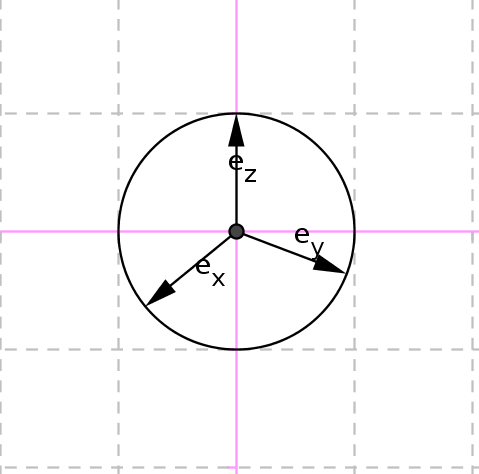
\includegraphics[scale=1]{unitvectors.png}
\caption{The three basis vectors point into the positive directions of the desired coordinate axis. They are arranged around a circle with the trigonometric functions of cosine and sine.}
\end{figure}

To reach all three (x,y) at the tips of the vectors, we will now pull out the cosine and sine functions and stuff them together
with $r$ and $\varphi$ into a 2x1 vector with two components. So any (x,y) on one line from the origin to far distance can be reached like in polar coordinates\footnote{Interested readers may find in \cite{Corral1}, \cite{Corral2} and \cite{Strang2} everything about polar coordinates, parametrization of x and y with cosine and sine, the unit circle and the distance or radius r and more to these topics.} with the following parametrization.\\

\begin{displaymath}
\left(\begin{array}{1}x\\y\end{array}\right) = \left(\begin{array}{1}r \cos \varphi\\ r \sin \varphi\end{array}\right)\\
\end{displaymath}\\

Which can alternativly it can be written like $(x,y) = (r \cos \varphi, r \sin \varphi)$.\\

Modeling the three two dimensional basis vectors with this information,
we get the following three two dimensional basis vectors. They point along the coordinate axes and are the ruler for our transformation.\\

\begin{displaymath}
\vec{e}_x := (r_x\cos(\varphi_x), r_x\sin(\varphi_x) )^T = \left(\begin{array}{1}r_x\cos(\varphi_x)\\r_x\sin(\varphi_x) \end{array}\right)\\
\end{displaymath}
\begin{displaymath}
\vec{e}_y := (r_y\cos(\varphi_y), r_y\sin(\varphi_y) )^T = \left(\begin{array}{1}r_y\cos(\varphi_y)\\r_y\sin(\varphi_y) \end{array}\right)\\
\end{displaymath}
\begin{displaymath}
\vec{e}_z := (r_z\cos(\varphi_z), r_z\sin(\varphi_z) )^T = \left(\begin{array}{1}r_z\cos(\varphi_z)\\r_z\sin(\varphi_z) \end{array}\right)\\
\end{displaymath}\\

Each component of (x,y,z) has now an own basis vector. By multiplying the cos terms for the x' and the sin terms for y' with the corresponding component of (x,y,z) and summing the three products up for each of x' and y', we directly obtain the right coordinate on the plane. All we would have to do is to connect the points again, or to fill the space between. 

\begin{figure}[ht]
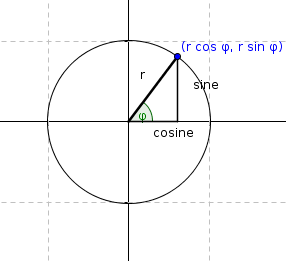
\includegraphics[scale=2]{unitcircle.png}
\caption{A picture of the unit circle, the hypotenuse r, the adjacent cosine, the opposite sine and the angle $\varphi$. It is a circle of radius r, and no longer the unit circle, if $r \neq 1$.}
\end{figure}

\subsection{About the vector basis lemma}\\

\subsubsection{The generic formula}

I am talking about multiplying the coordinates with the new vector basis, which i state to be the same as the coordinate system we drew on a piece of paper at the beginning. We wrote down the angles, made out the unit length, and wrote down the three basis vectors with the information. Where is this coming from?\\

Every mathematics, physics or related course has a lesson, where the orthogonal basis of an objects coordinate system is introduced. 
A orthogonal basis is a set of 2 or three or up to infinite orthogonal or perpendicular vectors. The describe a coordinate system, and one has to show for excercises, that the basis is linearly independent, that each basis vector points into it´s own dimension and not into the others.

The one lemma we need is the generic theorem for multiplying a vector with the vector basis for the target coordinate system.\\
In our case the orthogonality by 90 degrees rules do not count. The basis vectors are no longer perpendicular. And no longer completely linearly independent. 

\textbf{Remark} \emph{My move will be to show linear dependence by contradiction, and to call the basis a \textbf{pseudo-}basis then,
because of it´s correct result and wanted place in the hall of bases.}

The plane gives us two possible directions, to go horizontal or vertical. And in a cartesian coordinate system with infinite points, we can choose any direction around a center point (x,y). Which is in the case of our coordinate system the origin at (0,0,0) or (0,0). We will see later, that the zero vector stays in the origin for both systems.
Any not straight move will go horizontally or vertically by componentwise amounts. Any straight move horizontally or vertically will go by one of the components only.

The point is, the generic formula still holds.\\

Our pseudo basis is linearly dependent, but multiplying the coordinates with yield the right image of the set of points processed.\\

The formula for multiplying a vector with a base to get a new vector is this.\footnote{The formula can be found in many mathematics, chemistry and physics lecture scripts, and a good introduction is \cite{Strang1}.\\}

\begin{displaymath}
\vec{v} = \displaystyle\sum_{i=1}^{n} \vec{x}_i\vec{e}_i
\end{displaymath}

It is done componentwise for each row of the vector. $n$ is the number of the source dimensions. In our case it is $n = 3$. 
We are summing three products for each component of the new vector. Our old $\vec{x}$ is a $\vec{x} \in \mathbb{R}^3$.\\
With $\vec{x}_i$ as the coordinate component and $\vec{e}_i$ as the corresponding basis vector in the right component. 
$\vec{v}$ is the resulting new vector.  The new vector $\vec{v}$ is a $\vec{v} \in \mathbb{R}^2$.\\

\subsubsection{Connection to ijk-Notation}

This is also equal to

\begin{displaymath}
\vec{v} = x\vec{i} + y\vec{j} + z\vec{k}
\end{displaymath}

what also explains, what the ijk-Notation means. If you don´t use it already for determining determinants for
calculating cross products. It is for describing a vector. Don´t forget, our $i, j, k$ basis is two dimensional, 
because we draw on a 2-D plane like the computer screen or a piece of paper. \\

With a 3x3 basis the vector $x\vec{i} + y\vec{j} + z\vec{k}$ is equal to \left(\begin{array}{1}x'\\y'\\z'\end{array}\right)$. But with a 2x3 basis the vector $x\vec{i} + y\vec{j} + z\vec{k}$ is becoming  \left(\begin{array}{1}x'\\y'\end{array}\right)$\\


\subsection{Time to show the operation}

The operation of multiplying the (x,y,z) coordinate with our basis vectors in order is the following:\\

\begin{displaymath}
\left(\begin{array}{1}x'\\y'\end{array}\right) = \left(\begin{array}{1}
xr_x\cos(\varphi_x) + yr_y\cos(\varphi_y) + zr_z\cos(\varphi_z)\\
xr_x\sin(\varphi_x) + yr_y\sin(\varphi_y) + zr_z\sin(\varphi_z)\end{array}\right)\\
\end{displaymath}\\

Right, this small formula brings the unexpected 1:1 images of the preimage from $R^3$ to $R^2$.\\

What is new, what we know now? Each $(x,y,z)$ coordinate has to be multiplied with the vectors for the new $(x',y')$.
With the corresponding terms of the basis vectors for each of x,y,z in the matrix. That means,
to sum the products with $(x,y,z)$ and the cos terms up for $x'$ and to sum the products
of $(x,y,z)$ and the sin terms up for $y'$. This is the same as imagining walking left and
right with $\cos \varphi$ and up and down with $\sin \varphi$. Or mathematically adding positive or negative values to move up and down and left and right to the right spot. On the piece of paper, you take the ruler. You count the units, and go parallel to each axis. From the point you reached along parallel to the current axis as many units as the coordinate component has.

It is almost time to finish the matrix and to go through a set of points to draw the new set of resulting points.
For this i close the chapter and come to the part of the formal mathematical definitions.\\

\section{Theorem}

Let $V$ be the set of all points $(x,y,z) \in R^3$ which are about to become transformed. $V = \{ \vec{v}=(x,y,z) | x,y,z \in R^3 \}$.
Let $W$ be the set of all points $(x',y') \in R^2$ which are the result of the transformation $W = \{ \vec{w}=(x',y') | x',y' \in R^2, (x',y')=\boldsymbol{A}\vec{v}\}$.\\

\textbf{Remark} This chapter needs to be overworked with correct definitions of the sets, domain and range, etc.\\


\subsection{The transformation matrix}
\index{Definition}
\newtheorem{Definition}{Definition}
\begin{Definition}

Let \boldsymbol{A} be the matrix containing the three, two dimensional and trigonometric, basis vectors in order, one each
column. You get a rectangular 2x3 matrix $\boldsymbol{A} \in \mathbb{R}^{2x3}: \mathbb{R}^{3} \rightarrow \mathbb{R}^{2}$. With the basis vectors $\left(\begin{array}{1}r_n \cos \varphi_n\\r_n \sin \varphi_n\end{array}\right)$ in the three columns. 

\begin{displaymath}
\boldsymbol{A} := \begin{pmatrix}
    \vec{e}_x & \vec{e}_y & \vec{e}_z
    \end{pmatrix}
    = 
    \begin{pmatrix}
    r_x\cos(\varphi_x) & r_y\cos(\varphi_y) & r_z\cos(\varphi_z) \\
    r_x\sin(\varphi_x) & r_y\sin(\varphi_y) & r_z\sin(\varphi_z) \\
    \end{pmatrix}\\
\end{displaymath}\\

$\boldsymbol{A}$ should be treated as operator $\boldsymbol{\hat{A}} \in \mathbb{R}^{2x3} : \mathbb{R}^3 \rightarrow \mathbb{R}^2$. ($\vec{x}) \mapsto \boldsymbol{A}\vec{x}$. 

\end{Definition}\\


\textbf{Remark} This chapter needs to be overworked.

\subsection{The transformation}
\index{Theorem}
\newtheorem{Theorem}{Theorem (The Fundamental Theorem of transforming 3-D Points into 2-D Points)}
\begin{Theorem}\\

If you multiply \boldsymbol{A}, the matrix of the three two-dimensional basis vectors,
with the three-coordinate point $(x,y,z)$, the result is a two coordinate point, 
$(x',y')$. This point $(x',y')$ is the correct point on the two dimensional plane,
representing the point $(x,y,z)$ from the three dimensional coordinate system, you are transforming.\\

\begin{displaymath}
\boldsymbol{A}\left(\begin{array}{1}x\\y\\z\end{array}\right) = \left(\begin{array}{1}x'\\y'\end{array}\right)
\end{displaymath}

Applying the operator \boldsymbol{\hat{A}} transforms the point $(x,y,z) \in \mathbb{R}^3$ into a new point $(x',y') \in \mathbb{R}^2$. 

\textbf{Proof}:\\

\begin{displaymath}
\boldsymbol{A}\left(\begin{array}{1}x\\y\\z\end{array}\right) = x\vec{e}_x + y\vec{e}_y + z\vec{e}_z\\
%\end{displaymath}
%\begin{displaymath}
&= \left(\begin{array}{1}xr_x\cos(\varphi_x) + yr_y\cos(\varphi_y) + zr_z\cos(\varphi_z)\\
xr_x\sin(\varphi_x) + yr_y\sin(\varphi_y) + zr_z\sin(\varphi_z)\\
\end{array}\right) = \left(\begin{array}{1}x'\\y'\end{array}\right)
\end{displaymath}

\begin{figure}[ht]
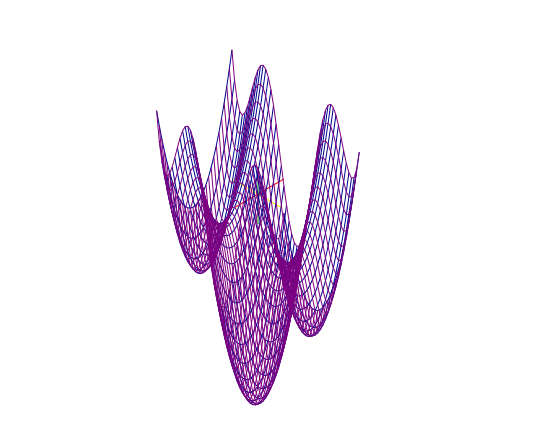
\includegraphics[scale=0.5]{fxyplot.png}
\caption{$f(x,y) = x^2 + y^2 + 3y \sin y$ from [-5,5] and [-3,3] on a Canvas2DRenderingContext}
\end{figure}


\end{Theorem}

\subsection{Computer implementations of the matrix and the transformation}
\subsubsection{Generic computer code}
\begin{example}
The following is example code for various computer systems.\\
\begin{lstlisting}
x_ = x*r*cos(alpha) + y*r*cos(beta) + z*r*cos(gamma)
y_ = x*r*sin(alpha) + y*r*sin(beta) + z*r*sin(gamma)
\end{lstlisting}
\end{example}\\


\subsubsection{JavaScript computer code}
\begin{example}
This is a full EcmaScript 6 snippet with all neccessary informations.\\
\begin{lstlisting}
let rad = (deg) => Math.PI/180*deg;
let r_x = 1, r_y = 1, r_z = 1; 
let phi_x = rad(220), phi_y = rad(330), phi_z = rad(90); 
let xAxisCos = r_x*Math.cos(phi_x), 
    yAxisCos = r_y*Math.cos(phi_y),
    zAxisCos = r_z*Math.cos(phi_z),
    xAxisSin = r_x*Math.sin(phi_x), 
    yAxisSin = r_y*Math.sin(phi_y),
    zAxisSin = r_z*Math.sin(phi_z);
let transform2d = ([x,y,z]) => [
    x*xAxisCos+ y*yAxisCos+ z*zAxisCos,
    x*xAxisSin+ y*yAxisSin+ z*zAxisSin];
let transform2dAll = (P) => P.map(transform2d);

let examplePoints = transform2dAll([[1,2,3], [3,4,5], [14,24,15]]);
\end{lstlisting}
\end{example}\\



\begin{figure}[ht]
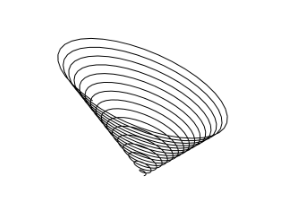
\includegraphics[scale=0.5]{conicalhelix.png}
\caption{A conical helix (t/2*Math.cos(t), t*Math.sin(t), t) shown as (x,y,z)=f(t) with implement.html on a Canvas2DRenderingContext testing the javascript example code.}
\end{figure}




\section{Corollary}

\subsection{Converting four Dimensions down to two dimensions}\\

The theorem can be used to handle more dimensions, for example can four two-dimensional
vectors represent a 4-D space on the 2-D plane. They get converted into the correct
2-D points. For Example, if you use a 2x4 matrix and convert all points at each 
instance of $t$ you have a moving object into the direction of the fourth basis vector. \\

\begin{displaymath}
\boldsymbol{A} := \begin{pmatrix}
    \vec{e}_x & \vec{e}_y & \vec{e}_z & \vec{e}_t\end{pmatrix}\\ = 
    \begin{pmatrix}
    r_x\cos(\varphi_x) & r_y\cos(\varphi_y) & r_z\cos(\varphi_z) & r_t\cos(\varphi_t)\\
    r_x\sin(\varphi_x) & r_y\sin(\varphi_y) & r_z\sin(\varphi_z) & r_t\sin(\varphi_t)\\
    \end{pmatrix}
\end{displaymath}

Here the basis is four times of two dimensions. A 2x4 matrix with four two dimensional basis vectors, one for each axis.\\

\begin{displaymath}
\boldsymbol{A}\left(\begin{array}{1}x\\y\\z\\t\end{array}\right) = \sum_{n} \vec{e}_n\vec{x}_n = \left(\begin{array}{1}x'\\y'\end{array}\right)\\
\end{displaymath}

\textbf{Proof}:

\begin{displaymath}
\boldsymbol{A}\left(\begin{array}{1}x\\y\\z\\t\end{array}\right) &= \left(\begin{array}{1}
xr_x\cos(\varphi_x) + yr_y\cos(\varphi_y) + zr_z\cos(\varphi_z) + zr_t\cos(\varphi_t)\\
xr_x\sin(\varphi_x) + yr_y\sin(\varphi_y) + zr_z\sin(\varphi_z)+ zr_t\sin(\varphi_t)\end{array}\right)\\
\end{displaymath}
\begin{displaymath}
&= x\vec{e}_x + y\vec{e}_y + z\vec{e}_z + t\vec{e}_t &= \sum_{n} \vec{e}_n\vec{x}_n &= \left(\begin{array}{1}x'\\y'\end{array}\right)
\end{displaymath}\\

The same method can be used to convert any other number of dimensions to the $xy$-plane. But it can also be
used in a generic m by n case\footnote{http://de.wikipedia.org/wiki/Abbildungsmatrix, also found in lecture scripts, but not anyone explaining me this matrix here or the topic of the from-three-to-two-points conversion. Is it too obvious? Or isn´t it obvious?}, to convert from n dimensions down to m, if you know the basis for the destination.\\

\section{Summary}

\subsection{Summary of all neccessary steps}
\begin{enumerate}
\item Lay out the three basis vectors around a circle and write down the angles $\varphi_n$. Programmers have to write down a variable for anyways.
\item Write down the basis vectors $\vec{e}_n$ as $r_n \cos \varphi_n$ and $r_n \sin \varphi_n$ (two dimensional). Don´t multiply with $r_n$ for a unit length of $1$ or multiply with $r_n$ to change the length of the basis vector.
\item Put the three basis vectors $\vec{e}_n$ into a matrix \bigsymbol{A}. Programmers can directly code the two lines of multiplication and forget the formal rest.
\item Iterate over your points and multiply each $(x,y,z)$ with the matrix \boldsymbol{A}, which acts as a linear operator, and put $(x',y')$ into your new set.
\end{enumerate}

\textbf{Remark}\\
About the word \emph{unit}. I am not really sure, if i have to use \emph{base vector} for a vector of any length and \emph{unit vector} only for the \emph{unit length} of $1$. Because of the misleading mismatch with the \emph{unit} of the thought \emph{coordinate axes}, which the \emph{base vector} defines, i tend in the first versions to misuse the word \emph{unit vector} for both. If you find this, or any other formal mistake, be sure, it is not wanted :-) I will try to remove more of these spelling errors\footnote{The \emph{Gerholdian operator}, the \emph{Gerholdian basis}, the \emph{Gerhold projection matrix}, the \emph{Gerhold transformation} are my favourite nicknames for my late discovery, making sure, the three two dimensional and trigonometric basis vectors, which i explained, sit in the matrix.} in the next versions.


\begin{thebibliography}    

    \bibitem{Corral1} \textit{Michael Corral, Schoolcraft College},
        Vector Calculus, GNU Free Documentation License, http://mecmath.net 
        
    \bibitem{Corral2} \textit{Michael Corral, Schoolcraft College},
        Trigonometry, GNU Free Documentation License, http://mecmath.net         
        
    \bibitem{Strang1} \textit{Gilbert Strang, MIT},
        Linear Algebra and it´s Applications. Fourth Edition.
        
    \bibitem{Strang2} \textit{Gilbert Strang, MIT},
            Calculus. MIT OpenCourseWare Supplemental Resources. http://ocw.mit.edu    
            
    \bibitem{Corral3} \textit{Michael Corral, Schoolcraft College},
            Latex Mini Tutorial, http://mecmath.net            
            
    \bibitem{Jürgens,Feuerstack} \textit{Manuela J\"urgens, Thomas Feuerstack, Fernuniversit\"at Hagen},
            LaTeX, eine Einf\"uhrung und ein bisschen mehr..., a026\_latex\_einf.pdf
            
    \bibitem{Rudl} \textit{Dr.Jan Rudl, Technische Universit\"at Dresden, Fachbereich Mathematik},
            Einf\"uhrung in LaTeX, LaTeX-Kurs.pdf            

\end{thebibliography}



\appendix

\section{Proving more rules of vector spaces}\\

\subsection{The origin stays in the origin}

A trivial proof is to prove, that the zero vector $\vec{0} \in \mathbb{R}^3$ maps to the zero vector $\vec{0} \in \mathbb{R}^2$.\\

\textbf{Proof}:
\begin{displaymath}
    \boldsymbol{A}\left(\begin{array}{1}0\\0\\0\end{array}\right)
    = \left(\begin{array}{1}0 + 0 + 0\\0 + 0 + 0\end{array}\right) 
    =\left(\begin{array}{1}0\\0\end{array}\right)
\end{displaymath}\\

\subsection{Points along one axis}

Another trivial proof is to prove, that coordinates lying on one axis are a multiple of the basis vector of the axis.\\

\textbf{Proof}:
\begin{displaymath}
    \boldsymbol{A}\left(\begin{array}{1}a\\0\\0\end{array}\right)
    = \left(\begin{array}{1}ar_x\cos \varphi_x + 0 + 0\\ar_x\sin \varphi_x  + 0 + 0\end{array}\right) 
    = a\vec{e}_x
\end{displaymath}

\begin{displaymath}
    \boldsymbol{A}\left(\begin{array}{1}0\\1\\0\end{array}\right)
    = \left(\begin{array}{1}0 + r_y\cos \varphi_y + 0\\0 + r_y\sin \varphi_y + 0\end{array}\right) 
    = \vec{e}_y
\end{displaymath}

\begin{displaymath}
    \boldsymbol{A}\left(\begin{array}{1}0\\0\\-b\end{array}\right)
    = \left(\begin{array}{1}0 + 0 - br_z\cos \varphi_z\\0 + 0 - br_z\sin \varphi_z\end{array}\right) 
    = -b\vec{e}_z
\end{displaymath}\\

\subsection{Multiplications with constants}

Another trivial proof is to show, that $\boldsymbol{A}(\lambda\vec{x}) = \lambda\boldsymbol{A}\vec{x}$. It doesn´t matter, where you multiply with the constant. You can multiply the original vector, or the resulting vector. You reach the same point.\\

\textbf{Proof}:\\
\begin{displaymath}
\begin{equation*}
\begin{align*}
\boldsymbol{A}(\lambda\vec{x}) &= \boldsymbol{A}\left(\begin{array}{1}\lambda{x}\\\lambda{y}\\\lambda{z}\end{array}\right)\\ &= \left(\begin{array}{1}\lambda{x}r_x\cos(\varphi_x) + \lambda{y}r_y\cos(\varphi_y) + \lambda{z}r_z\cos(\varphi_z)\\
\lambda{x}r_x\sin(\varphi_x) + \lambda{y}r_y\sin(\varphi_y) + \lambda{z}r_z\sin(\varphi_z)
\end{array}\right)\\
    &= \lambda\left(\begin{array}{1}xr_x\cos(\varphi_x) + yr_y\cos(\varphi_y) + zr_z\cos(\varphi_z)\\
xr_x\sin(\varphi_x) + yr_y\sin(\varphi_y) + zr_z\sin(\varphi_z)\\
\end{array}\right)\\
    &= \lambda\left(\begin{array}{1}x'\\y'\end{array}\right)\\
    &= \lambda\boldsymbol{A}\vec{x}
\end{align*}
\end{equation*}
\end{displaymath}\\


\subsection{Additions and subtractions}

Another trivial proof is to show, that $\boldsymbol{A}(\vec{v} + \vec{w}) = \boldsymbol{A}\vec{v} + \boldsymbol{A}\vec{w}$. 
It does not matter, if you add the original or the results . The outcome is the same point, the same vector.\\
 
\textbf{Proof}:\\

\begin{displaymath}
\begin{equation*}
\begin{align*}
\boldsymbol{A}\left(\begin{array}{1}x+u\\y+v\\z+w\end{array}\right) &= \left(\begin{array}{1}(x+u)r_x\cos(\varphi_x) + (y+v)r_y\cos(\varphi_y) + (z+w)r_z\cos(\varphi_z)\\
(x+u)r_x\sin(\varphi_x) + (y+v)r_y\sin(\varphi_y) + (z+w)r_z\sin(\varphi_z)\\
\end{array}\right)\\
            &= \left(\begin{array}{1}xr_x\cos(\varphi_x) + yr_y\cos(\varphi_y) + zr_z\cos(\varphi_z)\\
xr_x\sin(\varphi_x) + yr_y\sin(\varphi_y) + zr_z\sin(\varphi_z)\\
\end{array}\right) + \left(\begin{array}{1}ur_x\cos(\varphi_x) + vr_y\cos(\varphi_y) + wr_z\cos(\varphi_z)\\
ur_x\sin(\varphi_x) + vr_y\sin(\varphi_y) + wr_z\sin(\varphi_z)\\
\end{array}\right)\\    
    &= \left(\begin{array}{1}x'\\y'\end{array}\right) + \left(\begin{array}{1}u'\\v'\end{array}\right)\\
    &= \boldsymbol{A}\left(\begin{array}{1}x\\y\\z\end{array}\right) + \boldsymbol{A}\left(\begin{array}{1}u\\v\\w\end{array}\right)
\end{align*}
\end{equation*}
\end{displaymath}
\subsection{Rule of linearity}

\textbf{Corollary} From the previous two proofs, it is obvious to see, that
\begin{displaymath}
\boldsymbol{A}(\lambda\vec{v} + \kappa\vec{w}) = \lambda\boldsymbol{A}\vec{v} + \kappa\boldsymbol{A}\vec{w} = \lambda\left(\begin{array}{1}x'\\y'\end{array}\right) + \kappa\left(\begin{array}{1}u'\\v'\end{array}\right)\\
\end{displaymath}
which is a standard formulation of the rule of linearity. For example, you can find this rule in the form $\boldsymbol{A}(c\vec{x} + d\vec{y}) = c\boldsymbol{A}\vec{x} + d\boldsymbol{A}\vec{y}$ in \cite{Strang1}, but also in every linear algebra 1 lecture script.\\


\subsection{About the norm}

The norm used is the euclidean norm, or the 2-norm. This is the square root of the sum of the squares of the absolute values of the components $\|\vec{x}\| = \sqrt{\sum_{i=1}^{n}|x_n|^2}$. In linear algebra, functional analysis and topology lectures there are three fundamental properties of the norm. Definiteness, homogenity and the triangle inequality.\\


\textbf{Definitness} Show that $\|\vec{x}\| = 0$ if $\vec{x} = 0$\\
\begin{displaymath}
    \|\vec{x}\| = \|\vec{0}\| = \sqrt{0^{2} + 0^{2}} = 0
\end{displaymath}\\

\textbf{Homogenity} Show that $\|a\vec{x}\| = |a|\|\vec{x}\|$\\
\begin{displaymath}
    \|a\vec{x}\| = \sqrt{|a\vec{x}_1|^{2} + |a\vec{x}_2|^{2}} = \sqrt{|a|^{2}(|\vec{x}_1|^{2} + |\vec{x}_2|^{2})} = |a|\sqrt{|\vec{x}_1|^{2} + |\vec{x}_2|^{2}} = |a|\|\vec{x}\|
\end{displaymath}\\

\textbf{Triangle inequality} (Minkowski inequality) Show that $ \|\boldsymbol{A}(\vec{v} + \vec{w})\| \leq \|\boldsymbol{A}\vec{v}\| + \|\boldsymbol{A}\vec{w}\|$\\

\begin{displaymath}
    \sqrt{\sum_{i=1}^{n}|\vec{v}_i + \vec{w}_i|^{2}} \leq \sqrt{\sum_{i=1}^{n}|\vec{v}_i|^{2}} + \sqrt{\sum_{i=1}^{n}|\vec{w}_i|^{2}} 
\end{displaymath}\\

\textbf{Remark} This subsection is not complete.

\subsection{Metrics}

Where a norm is, there will be a metric induced.
The measurement of the distance between two points is defined by the d-function. It is the length of the difference vector between the two points.\\
\begin{displaymath}
    d(\vec{x}, \vec{y}) = \|\vec{x}-\vec{y}\| = \sqrt{\sum_{i=1}^{n}|\vec{x}_i-\vec{y}_i|^2}
\end{displaymath}

Metrics have three fundamental properties.
\begin{enumerate}
\item If the distance is zero, the vectors are equal.
\begin{displaymath}
d(x,y) = 0 \iff x = y
\end{displaymath}
\item It does not matter, whether you read $d(x,y)$ or $d(y,x)$, the number must be equal.
\begin{displaymath}
d(x,y) = d(y,x)
\end{displaymath}
\item The third one is the triangle inequality. Going over another point is always a step longer.
\begin{displaymath}
d(x,z) \leq d(x,y) + d(y,z) 
\end{displaymath}
\end{enumerate}


\textbf{Remark} This subsection is not complete and has to be continued. The point is to measure now the difference between the original coordinates and the new planar coordinates. $d(\vec{x}, \vec{y})_2 = \|\vec{x}-\vec{y}\|_2 \leq d(\vec{x}, \vec{y})_3 = \|\vec{x}-\vec{y}\|_3$ is my assumption which is not proven now.

\subsection{Transpose and unproven}

\textbf{Remark} Less trivial is to figure out, what the transpose and the products with the transpose and the inverse matrices of those products are good for. Our rectangular 2x3 basis matrix has a transponse. A 3x2 matrix. The products are $\boldsymbol{A}\boldsymbol{A}^T$, a 2 by 2 matrix, and $\boldsymbol{A}^T\boldsymbol{A}$, a 3 by 3 matrix. Today i will just show the transpose. \\

\begin{displaymath}
\left(
    \begin{array}{111}
    r_x\cos(\varphi_x) & r_y\cos(\varphi_y) & r_z\cos(\varphi_z) \\
    r_x\sin(\varphi_x) & r_y\sin(\varphi_y) & r_z\sin(\varphi_z) \\
    \end{array}
\right)^T
= \left(
    \begin{array}{11}
    r_x\cos(\varphi_x) & r_x\sin(\varphi_x)\\
    r_y\cos(\varphi_y) & r_y\sin(\varphi_y)\\
    r_z\cos(\varphi_z) & r_z\sin(\varphi_z) \\
    \end{array}
\right)
\end{displaymath}\\

Multiplying out the transposes yield the following forms.

\begin{displaymath}
\boldsymbol{A}\boldsymbol{A}^T = \begin{pmatrix} 
\sum_{i=1}^{3}r_n\cos\varphi_n & \sum_{i=1}^{3}r_n^2\cos\varphi_n\sin\varphi_n\\
\sum_{i=1}^{3}r_n^2\cos\varphi_n\sin\varphi_n & \sum_{i=1}^{3}r_n\sin\varphi_n
\end{pmatrix} = \begin{pmatrix}a & b\\b & c
\end{pmatrix}

You see, in the 2x2 matrix $\boldsymbol{A}\boldsymbol{A}^T$ is $a_{ij} = a_{ji}$. In the 3x3 matrix $\boldsymbol{A}^T\boldsymbol{A}$ is also $a_{ij} = a_{ji}$. I will abbreviate $\cos \varphi_n$ with $C_n$ and
$\sin \varphi_n$ with $S_n$.

\textbf{Remark} I have not compared with the sin(A+B) formulas.

\begin{displaymath}
\boldsymbol{A}^T\boldsymbol{A} = \begin{pmatrix} 
    C_x^2+S_x^2 & C_xC_y+S_xS_y & C_xC_z+S_xS_z\\
    C_yC_x+S_yS_x & C_y^2+S_y^2 & C_yC_z+S_yS_z\\
    C_zC_x+S_zS_x & C_zC_y+S_zS_y & C_z^2+S_z^2
\end{pmatrix}
= \begin{pmatrix}
    r_x^2 & a & b \\
    a & r_y^2 & c \\
    b & c & r_z^2 \\
\end{pmatrix}
\end{displaymath}

\textbf{Remark} I wrote down the formula for the 2x2 determinant and noticed, it´s getting hairy writing with bare hands. Using numeric software like FreeMat should be less stressing. Whether it makes sense to calculate the determinants and the inverses or
not, can not be told from looking at these matrices by a guy like me. This topic is continued in the next versions.

\textbf{Remark} Missing are $|\boldsymbol{A}\boldsymbol{A}^T|$ and $|\boldsymbol{A}^T\boldsymbol{A}|$ and $(\boldsymbol{A}\boldsymbol{A}^T)^{-1}$ and $(\boldsymbol{A}^T\boldsymbol{A})^{-1}$ and various tries to combine them to $P$, to $x^TAx$, and and.



\section{An alternative graphics algorithm}

\textbf{Remark} This section is new on July 10.

With the new information how to translate the coordinates, it is obvious, that we want to draw some graphics on our 2-D Canvas.
By doing so, i already found out a few interesting points of how to do this. Without homogenous coordinates or 4 by 4 matrices.\\

\subsection{Origin}  

Setting the origin is an easy task. Assuming, the regular origin is at (0,0,0) and (0,0), we just need to add the shift to the coordinate. You can shift the 3-D Origin or the 2-D Origin.\\
\begin{lstlisting}
x = Ox + x;
y = Oy + y;
z = Oz + z;
\end{lstlisting}

\subsection{Translation}

Translating the points is very easy without a 4 by 4 matrix. You simply add the translation vector to each point.\\

\begin{lstlisting}
x = Tx + x;
y = Ty + y;
z = Tz + z;
\end{lstlisting}

\subsection{Scaling}

To scale the object you just have to multiply with the constant. Reflecting, that it is no difference, whether you multiply
before or after the transformation, you can choose, what to scale, the 3-D or the 2-D object.\\

\begin{lstlisting}
x = Sx * x;
y = Sy * y;
z = Sz * z;
\end{lstlisting}

\subsection{Local 3x3 basis}

If you wish to introduce different units into different directions, you have to apply a local basis. Applying the local 3x3
basis to an object makes it rotatable with changed units. If you change the units of r on the projection, rotation may give unrealistic results since suddenly the object stretches to an unexpected size. \\

The matrix applied locally is a 3x3 matrix $\begin{pmatrix} xBX & yBX & zBX\\ xBY & yBY & zBY\\ xBZ & yBZ & zBZ\end{pmatrix}$.
For example is $\begin{pmatrix} 1 & 0 & 0\\ 0 & 1 & 0\\ 0 & 0 & 1\end{pmatrix}$ is an orthogonal standard basis and the result is the same as if you do not apply any basis to the object, as the assumed default coordinate system in $R^{3}$ is orthogonal.

\begin{lstlisting}
u = x, v = y, w = z;
x = u*xBX + v*yBX + w*zBX;
y = u*xBY + v*yBY + w*zBY;
z = u*xBZ + v*yBZ + w*zBZ;
\end{lstlisting}

This of course transform the object by the directions and the length of the three three dimensional basis vectors.


\subsection{Rotation}

Rotating the object can be done in three dimensional space by applying the regular rotation matrices

\begin{lstlisting}
    u = x, v = y, w = z;
    y = v * rotxcos - w * rotxsin
    z = v * rotxsin + w * rotxcos
    u = x, v = y, w = z;
    x = u * rotycos + w * rotysin;
    z = -u * rotysin + w * rotycos;
    u = x, v = y, w = z;
    x = u * rotzcos - v * rotzsin;
    y = u * rotzsin + v * rotzcos;
\end{lstlisting}

\textbf{Remark} I have to remove the substitution and write the whole thing out again. Next version.

\subsection{Code Example}

Last but not least here is a code snippet doing all the things together, showing you the order of transformation.


\printindex
\end{document}